\section{Main Results}\label{sec:results}

% Table: Overall accuracy across 4 LLM families × 8 backends.
% n = 100 questions. Bracketed numbers are 95% bootstrap confidence intervals
% (2,000 resamples).
\begin{table}[t]
\centering
\caption{Overall accuracy on 100 questions across four LLM families and eight
backends. Bracketed values are 95\% bootstrap confidence intervals
(2{,}000 resamples). Bold marks the best in-context surface form per LLM;
italics mark the best KG agent.}
\label{tab:overall-acc}
\small
\setlength{\tabcolsep}{4pt}
\begin{tabular}{l rrrr}
\toprule
Backend & HCX-32B-Think & Qwen3-235B & Llama-4-Scout & gpt-oss-120b \\
\midrule
\multicolumn{5}{l}{\emph{Production KG-RAG agents (Setting B: Qwen-Coder query agent)}} \\
\backendname{typedb}     & 58 [48, 68] & \emph{73} [64, 81] & 56 [46, 66] & \emph{68} [58, 77] \\
\backendname{neo4j}      & \emph{60} [50, 69] & 67 [58, 76] & \emph{65} [56, 74] & 65 [56, 74] \\
\midrule
\multicolumn{5}{l}{\emph{Reference baselines}} \\
\backendname{context} (production retrieval) & 79 [71, 87] & 80 [72, 88] & 76 [67, 85] & 79 [71, 87] \\
\backendname{closed\_book} (no retrieval) & 10 [4, 16] & 13 [7, 20] & 9 [4, 15] & 13 [6, 20] \\
\midrule
\multicolumn{5}{l}{\emph{In-context surface-form ablation (full-graph dump)}} \\
\backendname{C-TQL}      & 85 [78, 92] & 90 [84, 95] & 63 [54, 72] & \textbf{95} [90, 99] \\
\backendname{C-Cypher}   & 86 [79, 92] & 92 [86, 97] & 62 [53, 71] & 91 [85, 96] \\
\backendname{C-NL}       & \textbf{91} [85, 96] & \textbf{93} [88, 98] & \textbf{83} [75, 90] & 92 [86, 97] \\
\backendname{C-JSONLD}   & 89 [83, 95] & \textbf{93} [88, 98] & 67 [57, 76] & 92 [86, 97] \\
\bottomrule
\end{tabular}
\end{table}


Table~\ref{tab:overall-acc} reports overall accuracy on 100 questions
for the full $4\times 8$ matrix of LLM families and backends. Three
patterns emerge.

\subsection{Production KG agents underperform in-context surface forms}

Across every LLM family, the in-context surface forms outperform the
production KG agents. Mean accuracy of the four in-context tiers
exceeds mean accuracy of the two KG agents by 8.25 percentage points
(Llama-4-Scout, the smallest gap), 22.0 (Qwen3-235B), 26.0
(gpt-oss-120b), and 28.75 (HCX-32B-Think, the largest).
Figure~\ref{fig:kg-vs-incontext} visualizes the gap.

% Figure: KG agent (production) vs in-context surface forms.
% Mean of typedb+neo4j vs mean of C-TQL/Cypher/NL/JSONLD per LLM.
\begin{figure}[t]
\centering
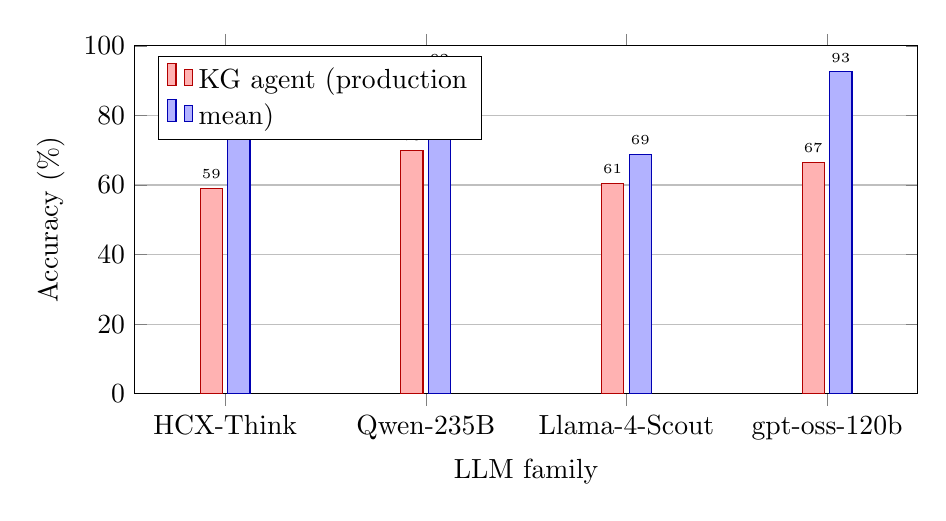
\begin{tikzpicture}
\begin{axis}[
  width=0.95\textwidth,
  height=6cm,
  ybar=2pt,
  bar width=8pt,
  ymin=0, ymax=100,
  ymajorgrids=true,
  ylabel={Accuracy (\%)},
  xlabel={LLM family},
  symbolic x coords={HCX-Think, Qwen-235B, Llama-4-Scout, gpt-oss-120b},
  xtick=data,
  legend pos=north west,
  legend cell align=left,
  enlarge x limits=0.15,
  nodes near coords,
  nodes near coords align={vertical},
  nodes near coords style={font=\tiny},
  every node near coord/.append style={/pgf/number format/.cd, fixed, precision=0},
]
% KG-agent mean = (typedb + neo4j) / 2
\addplot[fill=red!30, draw=red!70!black] coordinates {
  (HCX-Think, 59) (Qwen-235B, 70) (Llama-4-Scout, 60.5) (gpt-oss-120b, 66.5)
};
% In-context mean = (TQL + Cypher + NL + JSONLD) / 4
\addplot[fill=blue!30, draw=blue!70!black] coordinates {
  (HCX-Think, 87.75) (Qwen-235B, 92) (Llama-4-Scout, 68.75) (gpt-oss-120b, 92.5)
};
\legend{KG agent (production, mean), In-context surface form (mean)}
\end{axis}
\end{tikzpicture}
\caption{Production KG-RAG agents (mean of \backendname{typedb} and
\backendname{neo4j}) vs.\ in-context surface-form ablation
(mean of \backendname{C-TQL}, \backendname{C-Cypher}, \backendname{C-NL},
\backendname{C-JSONLD}). The in-context surface forms outperform the
production KG agents in all four LLM families, despite the KG agents
having access to a strictly larger graph (more entities and relations
than the dump). The gap ranges from 8 percentage points
(Llama-4-Scout, where the in-context tier is itself dragged down by KG
syntax familiarity) to 26 percentage points (gpt-oss-120b).}
\label{fig:kg-vs-incontext}
\end{figure}


This is counterintuitive in two ways. First, the KG agents
\emph{strictly} have access to more facts than the in-context dumps:
the production TypeDB and Neo4j stores contain entities that we did
not include in the in-context dumps (career tracks, allowance entities,
12 supplementary clauses, and three additional base-salary tables for
non-comprehensive-planning grades). Second, the KG agents are designed
exactly for multi-hop and multi-key queries — the regime in which the
in-context tiers should struggle most.

To test the gap rigorously we run paired McNemar exact two-sided
binomial tests on discordant pairs (Table~\ref{tab:mcnemar}). Of eight
KG-vs-context comparisons, five are statistically significant at
$p<0.05$ uncorrected, two are borderline ($p=0.052$), and only one
(Qwen-235B \backendname{typedb} vs \backendname{context}) fails to
reject the null. The win counts in the discordant column tell the
story: in HCX the KG agents win at most 5 questions while the context
agent wins 26.

% Table: McNemar paired tests for the main H1 (KG agent vs in-context).
% Exact two-sided binomial test on discordant pairs. n = 100 per cell.
\begin{table}[t]
\centering
\caption{Paired McNemar exact two-sided binomial tests over 100 paired
questions; only discordant pairs contribute to the statistic. Cell
format: ``$a$\,wins -- $b$\,wins'' counts the number of questions on
which only $a$ (resp. only $b$) is correct. Bold marks $p<0.05$.}
\label{tab:mcnemar}
\small
\begin{tabular}{l l c c}
\toprule
LLM & Comparison ($A$ vs $B$) & $A$ wins -- $B$ wins & $p$ \\
\midrule
\multirow{2}{*}{HCX-32B-Think}
 & \backendname{typedb} vs \backendname{context}   & 5 -- 26 & \textbf{0.0002} \\
 & \backendname{neo4j}  vs \backendname{context}   & 4 -- 23 & \textbf{0.0003} \\
\midrule
\multirow{2}{*}{Qwen3-235B}
 & \backendname{typedb} vs \backendname{context}   & 7 -- 14 & 0.189 \\
 & \backendname{neo4j}  vs \backendname{context}   & 5 -- 18 & \textbf{0.011} \\
\midrule
\multirow{2}{*}{Llama-4-Scout}
 & \backendname{typedb} vs \backendname{context}   & 3 -- 23 & \textbf{0.0001} \\
 & \backendname{neo4j}  vs \backendname{context}   & 5 -- 16 & \textbf{0.027} \\
\midrule
\multirow{2}{*}{gpt-oss-120b}
 & \backendname{typedb} vs \backendname{context}   & 8 -- 19 & 0.052 \\
 & \backendname{neo4j}  vs \backendname{context}   & 8 -- 22 & \textbf{0.016} \\
\bottomrule
\end{tabular}
\end{table}


\paragraph{Multiple-testing correction.}
The picture is consistent under family-wise control. Bonferroni
correction at $\alpha/8 = 0.00625$ leaves three comparisons significant
(HCX \backendname{typedb}, HCX \backendname{neo4j}, Llama-4
\backendname{typedb}). Holm--Bonferroni concurs. Benjamini--Hochberg
FDR control at $\alpha=0.05$ yields six significant comparisons,
additionally Qwen \backendname{neo4j} and Llama-4 \backendname{neo4j}.
The headline finding — production KG agents under-performing
in-context tiers — survives the most conservative family-wise
correction in three of four LLM families.

\subsection{The query-generation stage is the bottleneck, not KG expressivity}

The KG agents and the in-context dumps differ in exactly one
operational respect: the KG agents \emph{generate a query} (TypeQL or
Cypher) whose results they then verbalize, while the in-context dumps
hand the full graph directly to the chat model. Since the in-context
dumps preserve the same hyper-relational role-player structure
(C-TQL) or property-graph structure (C-Cypher) that the KG agents
exploit operationally, any drop in KG-agent accuracy must be
attributed to the additional pipeline stages: query authoring, query
execution, and result re-verbalization. The 8--26 percentage-point
gap therefore quantifies the cumulative loss of those stages — the
\emph{query-generation bottleneck}.

\subsection{Closed-book leakage is low}

The \backendname{closed\_book} baselines achieve 9--13\% on the same
100 questions, with a four-LLM mean of 11.25\%. This bounds the
contribution of pre-training memorization to RAG performance: the
75--80 point gap between any RAG-style backend and
\backendname{closed\_book} is genuine retrieval, not regurgitation
of memorized facts.

\subsection{Natural-language summary Pareto-dominates structured surface forms}

Among the in-context tiers, C-NL achieves the highest mean accuracy
(89.8\% across LLMs) at less than half the token cost of the
structured tiers (14K characters vs.\ 26--32K).
Table~\ref{tab:token-cost} and Figure~\ref{fig:pareto} display the
trade-off.

% Table: Surface-form size comparison (token efficiency frontier).
\begin{table}[t]
\centering
\caption{Surface-form size and mean accuracy across four LLM families.
C-NL Pareto-dominates the other in-context tiers: highest mean accuracy
at less than half the token cost.}
\label{tab:token-cost}
\small
\begin{tabular}{l r r}
\toprule
Surface form & Size (chars) & Mean accuracy \\
\midrule
C-MD (production retrieval, chunked) & $\sim$13K & 78.5\% \\
C-TQL (TypeQL insert dump)            & 32{,}436 & 83.3\% \\
C-Cypher (Cypher CREATE dump)         & 32{,}030 & 82.8\% \\
\textbf{C-NL (natural-language summary)} & \textbf{14{,}000} & \textbf{89.8\%} \\
C-JSONLD (nested JSON-LD)             & 26{,}278 & 85.3\% \\
\bottomrule
\end{tabular}
\end{table}

% Figure: Accuracy vs token cost — Pareto frontier shows C-NL dominates.
\begin{figure}[t]
\centering
\begin{tikzpicture}
\begin{axis}[
  width=0.85\textwidth,
  height=6cm,
  xlabel={Surface-form size (characters)},
  ylabel={Mean accuracy across four LLMs (\%)},
  xmin=10000, xmax=35000,
  ymin=75, ymax=95,
  ymajorgrids=true,
  xmajorgrids=true,
  scatter/classes={
    md={mark=triangle*, mark size=4pt, blue!50!black},
    tql={mark=square*, mark size=4pt, red!70!black},
    cy={mark=square*, mark size=4pt, orange!80!black},
    nl={mark=*, mark size=5pt, green!50!black},
    jsonld={mark=square*, mark size=4pt, purple!70!black},
  },
]
\addplot[scatter, only marks, scatter src=explicit symbolic,
  point meta=explicit symbolic, nodes near coords*={\labelname}, every node near coord/.append style={font=\small, anchor=west, xshift=8pt}]
table[meta=label]{
x      y     label    \labelname
13000  78.5  md       C-MD
32436  83.3  tql      C-TQL
32030  82.8  cy       C-Cypher
14000  89.8  nl       C-NL
26278  85.3  jsonld   C-JSONLD
};
\end{axis}
\end{tikzpicture}
\caption{Accuracy versus surface-form size (characters), averaged across
four LLM families. C-NL Pareto-dominates the structured surface forms:
highest mean accuracy at less than half the token cost. C-MD (production
chunked retrieval) under-performs full-graph dumps because retrieval
loses some context; the structured dumps (TQL, Cypher, JSON-LD) gain
nothing for their ~2.3$\times$ token overhead.}
\label{fig:pareto}
\end{figure}


The structured tiers (TQL, Cypher, JSON-LD) bring no accuracy benefit
proportional to their token overhead. The single exception —
gpt-oss-120b on C-TQL at 95\% — does not generalize: Llama-4-Scout
falls to 63\% on the same surface form, dragging down the C-TQL
mean. C-NL is the only surface form that maintains $\geq 83\%$
accuracy across all four LLMs.

\subsection{On Setting A vs.\ Setting B}

A 30-question pilot under \emph{Setting A} — same LLM as chat and
query agent — produced LLM-family-asymmetric KG results: Qwen3-235B
on \backendname{neo4j} jumped +23\,pp from Setting A to Setting B,
while \backendname{typedb} dropped --6\,pp. The asymmetry confirms
that single-LLM measurements conflate KG-backend effects with the
LLM's TypeQL/Cypher syntax familiarity, which is precisely the
mechanism Section~\ref{sec:mechanism} dissects. We therefore use
Setting B (query agent fixed at Qwen3-Coder-30B) as the
production-realistic configuration throughout this paper. Full
Setting A figures appear in Appendix~\ref{sec:appendix}; we report
them transparently rather than as a contrast that flatters the
main result.

\subsection{Multi-key categories: the regime KG agents are designed for}

Restricting to the H1-relevant categories — \texttt{calculation},
\texttt{comparison}, \texttt{multihop\_3key} (42 questions total) —
sharpens the picture: the KG agents range from 47.6\% to 66.7\%
on this subset (mean 57\%) while the in-context tiers reach
57.1\%--100\% (mean 90\%). The regime that hyper-relational KGs are
operationally tailored for is precisely where the in-context
full-graph dumps win largest, with per-LLM multi-key gaps of
17.9, 32.7, 39.9, and 41.7 percentage points (Llama-4-Scout,
Qwen3-235B, HCX-32B-Think, gpt-oss-120b respectively).
